\documentclass{article}
\usepackage[utf8]{inputenc}

\title{PICO 500: Optical Simulation for straight viewports}
\author{Jhoel Montes Palma }
\date{\today}

%Codification -------------------------------------------
\usepackage[utf8]{inputenc}
\usepackage[T1]{fontenc}
\usepackage{amsmath}
\usepackage{graphicx}
\usepackage{subcaption}
\usepackage{comment}

%Beginning---------------------------------------------------
\begin{document}

\maketitle

\section{Introduction}

\section{Position of cameras}

The methodology that I am going to follow in order to find the best position for the cameras in a particular configuration is the following:

\begin{itemize}
  \item We have to be able to see the entire fiducial volume of the detector (except the parts that can't be illuminated by the retroreflectors)
  \item The fiducial volume have to occupy the majority of the area in every image, so the focal length (which determines the angle of vision) of the cameras have to be maximal (minimum angle of vision). This ensures that most of the pixels are getting useful images to analyse.
  \item The overlap of the images from two cameras in the same vertical line has to be minimum so each camera focuses on its own part of the detector.
\end{itemize}

In the end, this maximum focal length is going to set a desirable value, rather than the exact value, this because of some possible technical issues that may restrict its value.

For simplicity I'm going to assume the following constraints:

\begin{itemize}
    \item All the cameras have the same focal lengths
    \item The radial distortion (barrel or pincushion distortion) is set to zero.
    \item The parts of the detector outside the bubble chamber that can't be seen with the cameras will be constructed roughly in the simulation.
    \item All the simulation are made just for two cameras in the same vertical line as the other two are symmetrical.
\end{itemize}

Following these conditions, we can obtain the optimal positions for the cameras.




\section{Explanation of output figures and one example}


First, for explanation purposes, we are going to run the simulation for the current configuration of the detector(without raytracing analysis) (figure \ref{fig:drawing}) with the same position of the cameras shown there.

In order to have a better analysis I am going to include a simple design for the retroreflector (one cone-section at the top of the detector)


\begin{figure}
    \centering
    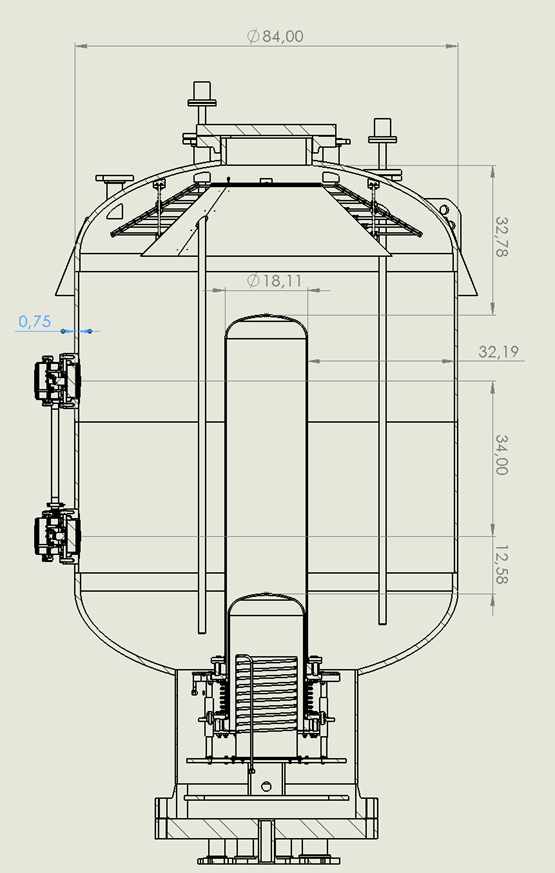
\includegraphics[width=8cm]{current_drawing.png}
    \caption{Caption}
    \label{fig:drawing}
\end{figure}

The parameters for this first simulation are listed in the table 

\begin{table}[]
    \centering
    \begin{tabular}{|c|c|}
        \hline
        top camera Z coordinate &  188.3 cm\\
        \hline
        bottom camera Z coordinate & 102.0 cm\\
        \hline
        separation betwen cameras & 86.3 cm\\
        \hline
        focal length & 0.8 cm\\
        \hline
        
    \end{tabular}
    \caption{Parameters of the first simulation. The z=0 plane is located at the base of the inner vessel.}
    \label{tab:my_label}
\end{table}


The first output of the raytracing code is a figure called "Y-Z cross section". This figure shows the scattering of the rays in the Y-Z cross section of the detector.

As we can see in figure , the rays cover the entire fiducial volume but many rays also hit other non useful parts (for analysis purposes) of the detector like the copper ring (bottom camera), the retroreflector (top camera) and even some rays go through the inner vessel and hit the parts below the copper ring (there's no retroreflector there so these rays do not come back to the camera).


The second output is a simulated image of the detector (figure=== ) as the camera sees it. The colors in the image are chosen randomly since there's no wavelength information in the raytracing code, but it provides a good perspective since every color shown in the figure represents a different set of surfaces where the rays have pass through

This figure reaffirms the fact that there are many rays (pixels in this figure) that haven't pass through the active volume of the detector.

Another useful figure is the cut-c3f8+retro figure which indicates which pixels of the image have pass trough the active liquid c3f8 and also has hit the retroreflector. This figure is shown in figure ( ) where we can see that in both images we can reduce the vision of the cameras (increase focal lenght) and still be able to see the entire fiducial volume(in blue).



\begin{figure}
    \centering
    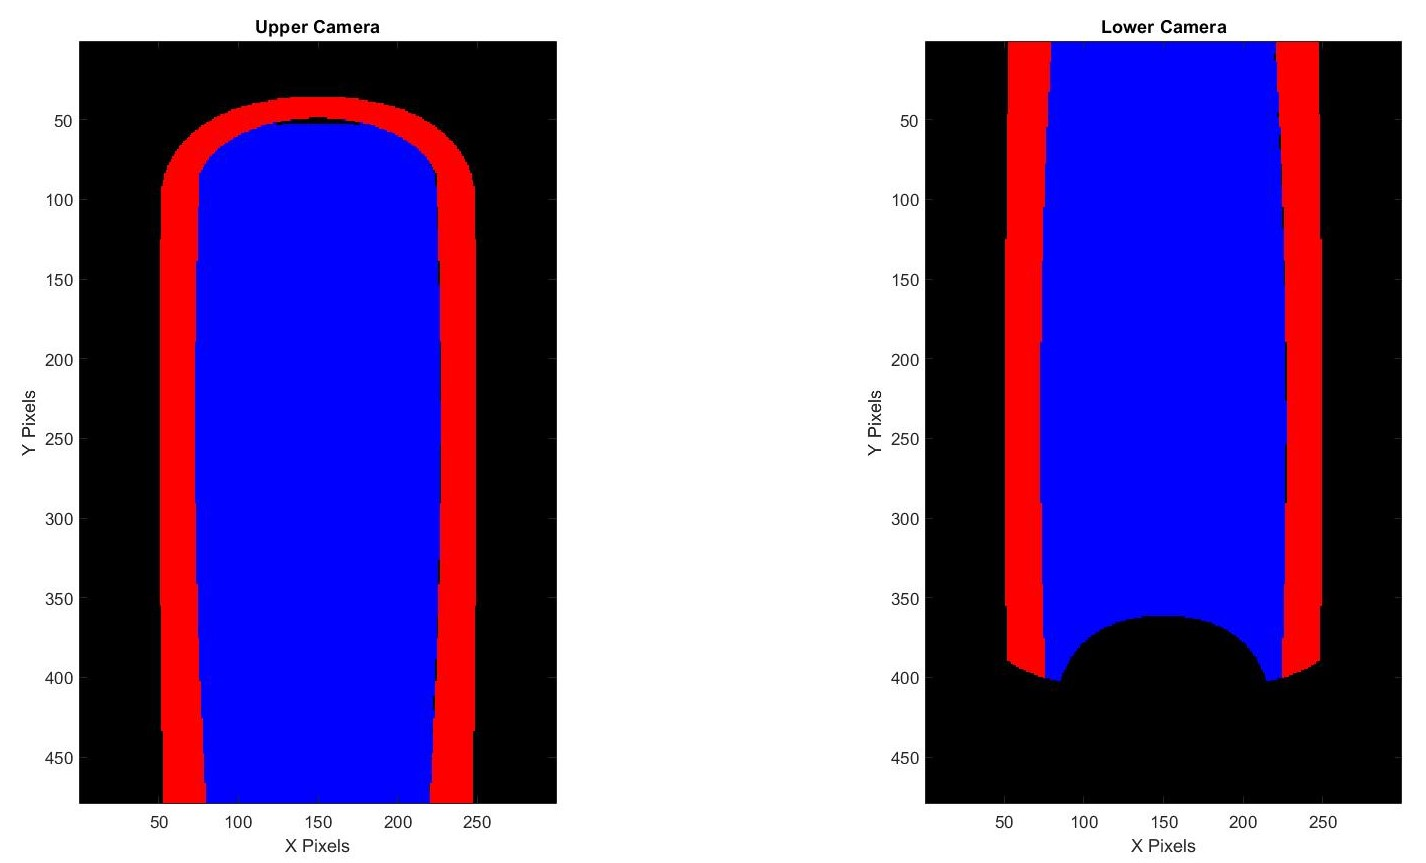
\includegraphics[width=12cm]{cut_c3f8+retro_copper_over_cyl_IIV_original_mathieu.jpg}
    \caption{Caption}
    \label{fig:my_label}
\end{figure}

Finally, the last figure that is going to help us to find the best positioning for the cameras is the surface-intersection figure, which shows all the surfaces where the rays have got in and out of the chamber, so we can ensure that all the fiducial volume is cover by the rays (specially at the intersection). In this case we can reduce a little bit more the overlap between the images.



\section{Best positioning}

\subsection*{Current Configuration}
By applying the discussed changes to the parameters we can get the optimal positions and focal length for the cameras.

The optimal parameters for the configuration shown in figure (mathieu) are:

\begin{table}[]
    \centering
    \begin{tabular}{|c|c|}
        \hline
        top camera Z coordinate &  188.3 cm\\
        \hline
        bottom camera Z coordinate & 102.0 cm\\
        \hline
        separation betwen cameras & 86.3 cm\\
        \hline
        focal length & 0.8 cm\\
        \hline
        
    \end{tabular}
    \caption{Parameters of the first simulation. The z=0 plane is located at the base of the inner vessel.}
    \label{tab:my_label}
\end{table}




hjhvjh






\end{document}
